\subsection{Vision}
As shown in the results section the image processing algorithm developed was able to find matching cards irrespective of changes in card orientations. There were a number of pitfalls to the vision detection algorithm.
One such unforseen pitfall was that we hadn't considered (initially) the possibility of trying to read a card when the arm had failed to pick it up in the first place which results in an image similar to Figure \ref{nocard} or in Figure \ref{cardStrug} which meant that some of our bounding box factors couldn't be fored, causing certain variables to be null which created an uncharacteristically abrupt failure to the system. By being able to adjust this (setting conditional default values) we managed to alter the system to be able to recognise that it had not identified any card, allowing us to handle that error and exit gracefully from the program.

\begin{figure}[position = here]
	\begin{centering}
		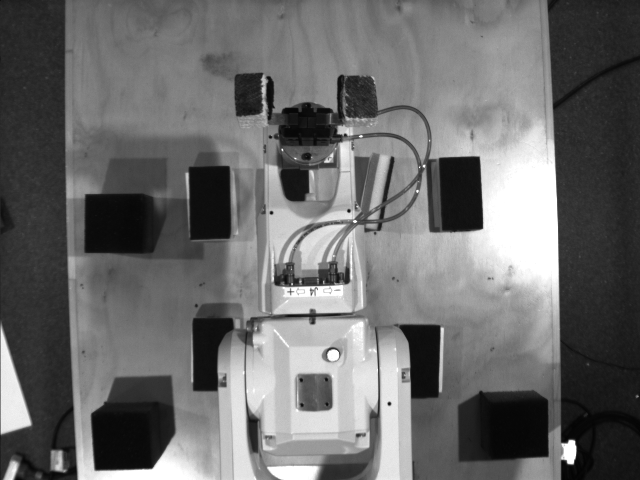
\includegraphics[scale=0.3]{./test_images_gray/test_image74.png}\\
		\caption[]{\textit{Failure to pick up a card\label{nocard}}}
	\end{centering}
\end{figure}

\begin{figure}[position = here]
	\begin{centering}
		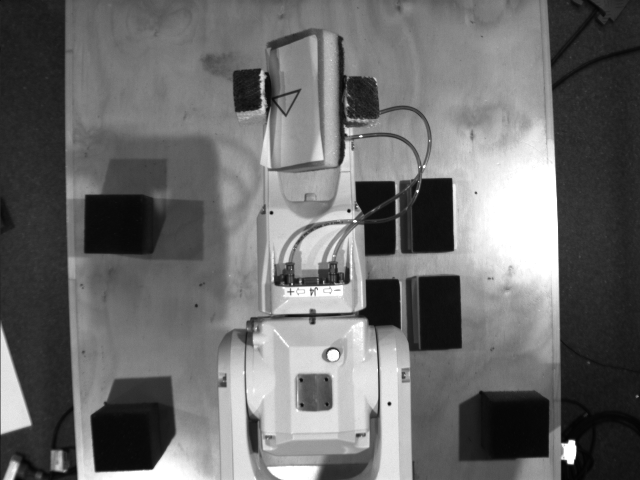
\includegraphics[scale=0.3]{./test_images_gray/test_image54.png}\\
		\caption[]{\textit{Struggling to hold the card properly\label{cardStrug}}}
	\end{centering}
\end{figure}

Shadows caused by the sponges themselves (and the manipulator arm) were found to affect our ability to properly estimate the position of the cards. This is, in part, because we could not automatically manipulate the thresholds to remove shadows. This is particularly observable under dull lighting conditions when the shadow's pixel representation is similar to the back of the card and can be solved by obtaining an RGB image (which was subject to the aforementioned issues with the camera driver) and conderting it into HSV format and nullifying shadow effects. It could also be solved by removing the structures taht created the shadows (such as the sponges) by changing the end effector to work without the sponges because the cards then would be smaller and thinner, thus minimising shadow that they create. However the shadow of the manipulator arm itself is a constant issue and an alternate lighting arrangement could balanced light source by providing light in multiple directions to minimise the shadows (similar to the effect of multiple floodlights on a sports field).